\section*{Parte 2}

Considere el sistema de control realimentado mostrado en la \href{figdb}{Figura 2}

\begin{figure}[!h]
    \centering
    \tikzstyle{block} = [draw, fill=white, rectangle, 
    minimum height=3em, minimum width=4em, node distance=2cm]
    \tikzstyle{gain} = [draw, fill=white, rectangle, 
    minimum height=3em, minimum width=2em, node distance=2cm]
    \tikzstyle{sum} = [draw, fill=white, circle, minimum size=15pt, node distance=2cm]
    \tikzstyle{input} = [coordinate]
    \tikzstyle{output} = [coordinate]
    \tikzstyle{pinstyle} = [pin edge={to-,thin,black}]
    \begin{tikzpicture}[auto, node distance=3cm]
       \node [input, name=input]{};
       \node [sum, right of=input](sum1){};
       \node [block, right of=sum1](controlador){$C(s)$};
       \node [sum, right of=controlador](sum2){};
       \node [block, right of=sum2](proceso){$P(s)$};
       \node [output, right of=proceso](output){};
        \node [input, above of=sum2, yshift=-4em](perturbación){};

       \draw [-{Latex}] (input) -- (sum1) node[name=r, midway, above]{$r(s)$};
       \draw [-{Latex}] (sum1) -- (controlador) node[name=error, midway, above]{$e(s)$};
       \draw [-{Latex}] (controlador) -- (sum2) node[name=control, midway, above]{$u(s)$};
       \draw [-{Latex}] (sum2) -- (proceso) node[name=lmao, midway, above]{};
       \draw [-{Latex}] (proceso) -- (output) node[name=y, midway, above]{$y(s)$};
       \draw [-{Latex}] (y) -- ++(0,-5em) coordinate (ort) -- (ort) -- (ort-|sum1) -- (sum1);
       \draw [-{Latex}] (perturbación) node[above]{$d(s)$} -- (sum2);

        \node [above left=-4pt of sum1]{$+$};
        \node [below left=-4pt of sum1]{$-$};
        \node [above right=-4pt of sum2]{$+$};
        \node [below left=-4pt of sum2]{$+$};
    \end{tikzpicture}
    \caption{Sistema de control realimentado}
    \label{figdb}
\end{figure}



\begin{itemize}
\item (20 pts) Simule el lazo de control ante cambios de tipo escalón unitario en el valor
deseado y en la perturbación considerando que el \textbf{proceso controlado es integrante
de segundo orden con ganancia unitaria, constante de tiempo de 0,2 segundos y
sin tiempo muerto} \textit{(sugerencia: repasar definición de este sistema en el capítulo 5 del
folleto de análisis de sistemas).}

Considere que el controlador está dado por $C(s) = K_p = 1$.

Recuerde que cuando se aplica un cambio en una entrada (ej. $r(t)$), se debe dar el
tiempo suficiente para que el sistema se estabilice y luego se aplica el cambio en la
siguiente entrada (ej. $d(t)$). Coloque en la memoria de su solución una imagen de la
respuesta del sistema de control $y(t)$ que también incluya las señales asociadas
al valor deseado $r(t)$ y a la perturbación $d(t)$. En una segunda imagen debe mostrar
el valor de la señal de control $u(t)$ ante los mismos cambios aplicados en las entradas
del sistema. Ambas figuras deben incluir las entradas de referencia y perturbación, y
presentarse con una descripción de los ejes usando el comando \texttt{xlabel}, \texttt{ylabel} y una
leyenda (\texttt{legend}). El fondo de las figuras debe ser blanco, y el grosor de las líneas
mostradas en cada figura debe ser el adecuado tal que permita fácilmente identificar
cada señal.

\vspace{1em}

    \textit{Solución.} En base a la descripción del modelo del proceso indicado en el enunciado, se implementó en MATLAB la siguiente función de transferencia
\begin{align*}
    P(s) = \frac{1}{s(0.2s+1)}
\end{align*}

Lo cual se implementó en MATLAB de la siguiente manera:

\vspace{1em}

\begin{mdframed}
\begin{minted}{matlab}
...
s = tf('s');

Kp = 1;
K = 1;
L = 0;
T = 0.2;

P = K * exp(-L*s)/(1+T*s);
C = Kp;
...
\end{minted}
\end{mdframed}

Además de esto, se analizó el comportamiento del sistema cuando $r(t) = \mu(t-1)$ y $d(t) = \mu(t-6)$ para esta simulación y el resto que se mostrarán más adelante. Esto en MATLAB, se genera de la siguiente forma

\vspace{1em}
\begin{mdframed}
\begin{minted}{matlab}
...
r = 0;
r ( t >= 1) = 1;
d = 0; 
d ( t >= 6) = 1;
...
\end{minted}
\end{mdframed}

La respuesta del sistema $y(s)$ posee una parte de servocontrol ($d(s) = 0$) y reguladora ($r(s) = 0$). Esto se expresa de la siguiete forma:
\begin{align*}
    y(s) =\underbrace{M _{yr}(s)r(s)}_{\text{Servocontrol}} + \underbrace{M _{yd}(s)d(s)}_\text{{Regulador}}
\end{align*}

Donde $M _{yr}(s)$ y $M _{yd}(s)$ se definen de la siguiente manera:
\begin{align*}
    M _{yr}(s) &= \frac{C(s)P(s)}{ 1 + C(s)P(s)}\\
    M _{yd}(s) &= \frac{P(s)}{ 1 + C(s)P(s)}
\end{align*}
Y en particular, se cumple la siguiente relación
\begin{align*}
    M _{yr}(s) = C(s)M _{yd}(s)
\end{align*}
Para la señal de control $u(s)$, se tiene una parte de servomecanismo, y una parte reguladora. De forma similar a la respuesta del sistema $y(s)$, se tiene:
\begin{align*}
    u(s) =\underbrace{M _{ur}(s)r(s)}_{\text{Servomecanismo}} + \underbrace{M _{ud}(s)d(s)}_\text{{Regulador}}
\end{align*}

Donde $M _{ur}(s)$ y $M _{ud}(s)$ se definen de la siguiente manera:
\begin{align*}
    M _{ur}(s) &= \frac{C(s)}{ 1 + C(s)P(s)}\\
    M _{ud}(s) &= \frac{-C(s)P(s)}{ 1 + C(s)P(s)}
\end{align*}
Y en particular, se cumple la siguiente relación
\begin{align*}
    M _{ur}(s) = -P(s)M _{ud}(s)
\end{align*}
Para la implementación en MATLAB, se tuvo que utilizar la función \texttt{minreal} para garantizar la cancelación de polos y ceros, ya que esto puede ser un problema debido a la cantidad de cifras significativas que MATLAB utiliza para el almacenamiento de estos parámetros. A continuación se muestr a el código correspondiente
\vspace{1em}
\begin{mdframed}
\begin{minted}{matlab}
t = 0:0.01:10;
...
MydA = minreal(P/(1+ C * P));
MyrA = minreal(MydA * C);

MurA = minreal(C/(1+ C * P));
MudA = minreal(MydA * -P);
...
yrA = lsim(MyrA, r ,t);
ydA = lsim(MydA ,d ,t );
yA = yrA + ydA;

urA = lsim(MurA, r ,t);
udA = lsim(MudA ,d ,t );
uA = urA + udA;
\end{minted}
\end{mdframed}
Por último, se realizaron las gráficas solicitadas en el enunciado. Esto se implementó en MATLAB por medio de los siguientes comandos:

\vspace{1em}
\begin{mdframed}
\begin{minted}{matlab}
figure (1) ;
x1=xlabel ('$t$ [s]');
hold on;
plot (t , yA, ...
    'LineWidth', 2.5, ...
    'Color', 'r');
plot (t , d, '--', ...
    'LineWidth', 2.5, ...
    'Color', 'b');
plot (t , r, '--', ...
    'LineWidth', 2.5, ...
    'Color', 'k');
grid on;
leg1=legend('$y(t)$', '$d(t)$', '$r(t)$');
set(x1,'Interpreter','latex');
set(x1,'FontSize',12);
set(leg1,'Interpreter','latex');
set(leg1,'FontSize',12);
hold off;

figure (2) ;
x2=xlabel ('$t$ [s]');
hold on;
plot (t , uA, ...
    'LineWidth', 2.5, ...
    'Color', 'r');
plot (t , d, '--', ...
    'LineWidth', 2.5, ...
    'Color', 'b');
plot (t , r, '--', ...
    'LineWidth', 2.5, ...
    'Color', 'k');
grid on;
leg2=legend('$u(t)$', '$d(t)$', '$r(t)$');
set(x2,'Interpreter','latex');
set(x2,'FontSize',12);
set(leg2,'Interpreter','latex');
set(leg2,'FontSize',12);
hold off;
\end{minted}
\end{mdframed}
Del código anterior, se obtuvieron las siguientes gráficas:

\begin{figure}[!h]
    \centering
    \begin{minipage}{0.45\linewidth}
        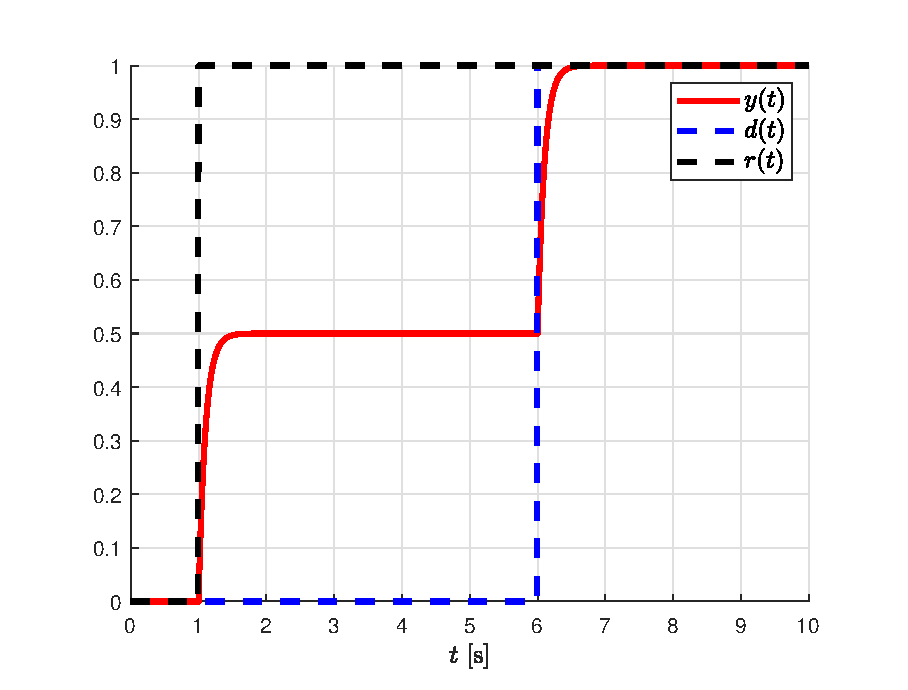
\includegraphics[width=\linewidth]{figs/fig2.eps}
        \caption*{(a): Respuesta del sistema}
    \end{minipage}
    \begin{minipage}{0.45\linewidth}
        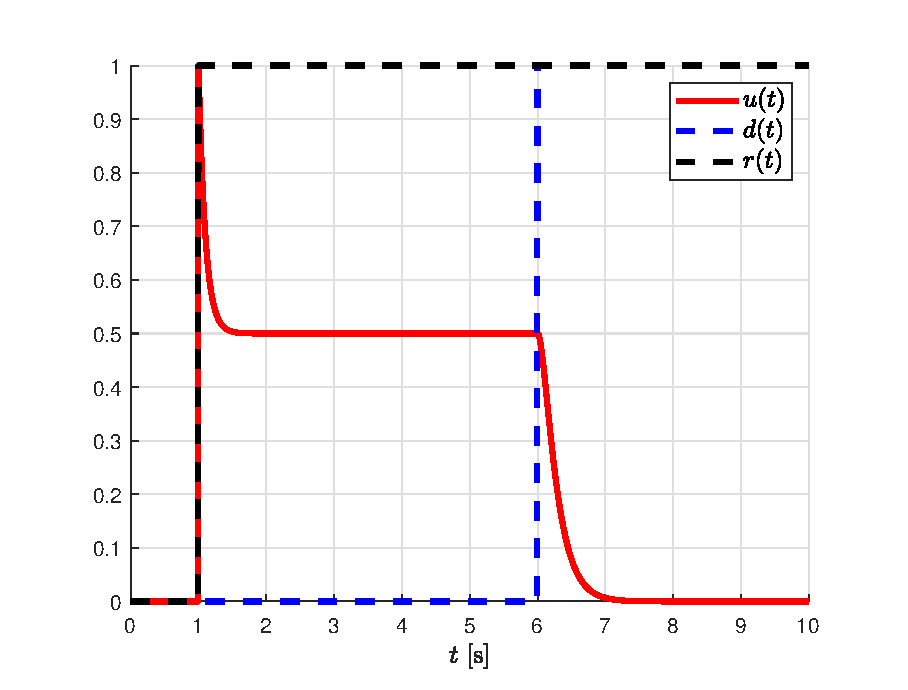
\includegraphics[width=\linewidth]{figs/fig3.eps}
        \caption*{(b): Respuesta del controlador}
    \end{minipage}
    \caption{Señales del sistema de control realimentado con $C(s) = 1$ y un proceso integrante de segundo orden}
    \label{fig3}
\end{figure}
De esta misma manera se generaron el resto de gráficas de esta tarea. No se listará más código repetido de MATLAB en la tarea, y solo aquel código nuevo que merezca una explicación.
\end{itemize}

\begin{itemize}
\item (20 puntos) Realice la misma simulación del punto anterior (incluyendo dos nuevas
imágenes asociadas a $y(t)$ y $u(t)$ con los mismos requerimientos y cambios aplicados en
$r(t)$ y $d(t)$), pero considerando que ahora el controlador está dado por:

\begin{align*}
    C(s) = K_P \left( 1 + \frac{1}{T_i s} \right) 
\end{align*}

donde $K_P = 2$ y $T_i = \SI{2}{s}$

\textit{Solución.} Para definir el controlador integrante utilizado en este inciso, se utilizó el siguiente código de MATLAB
\vspace{1em}
\begin{mdframed}
\begin{minted}{matlab}
...
C = Kp*(1+ 1/(Ti * s));
...
\end{minted}
\end{mdframed}
Al realizar la simulación del sistema realimentado, se obtuvieron las siguientes gráficas:

\begin{figure}[!h]
    \centering
    \begin{minipage}{0.45\linewidth}
        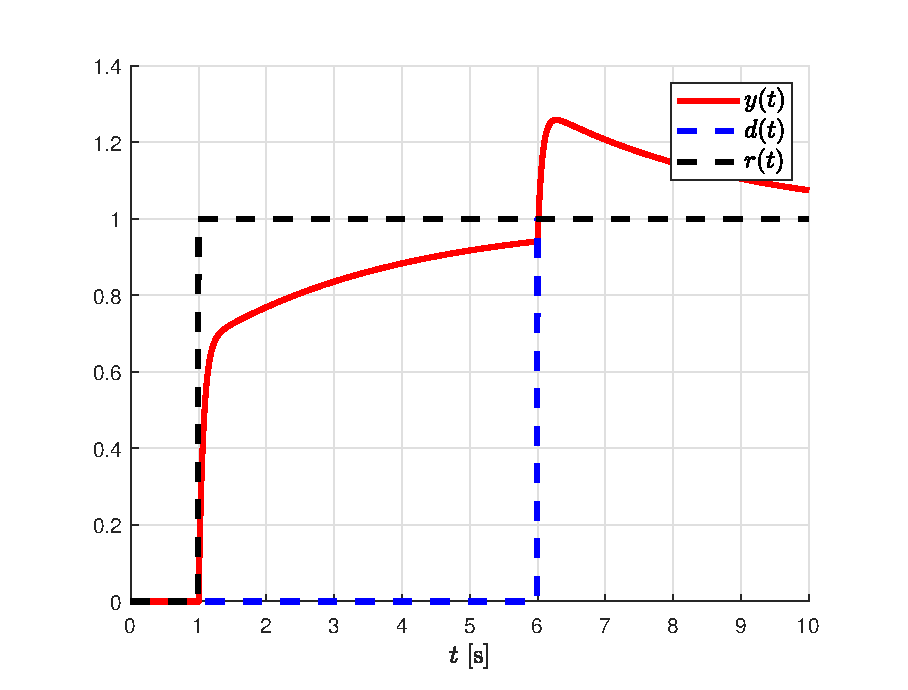
\includegraphics[width=\linewidth]{figs/fig4.eps}
        \caption*{(a): Respuesta del sistema}
    \end{minipage}
    \begin{minipage}{0.45\linewidth}
        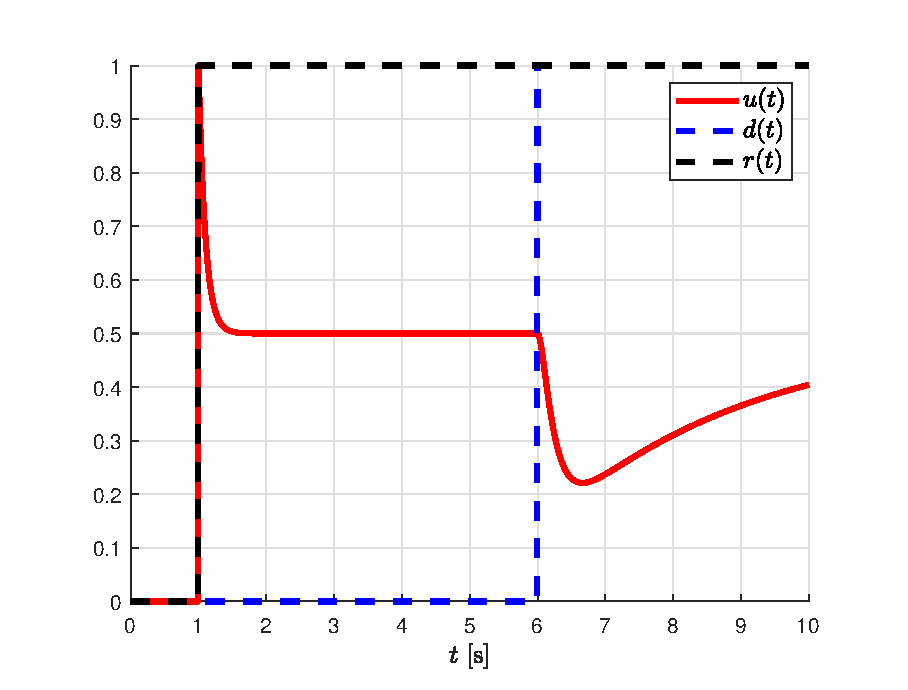
\includegraphics[width=\linewidth]{figs/fig5.eps}
        \caption*{(b): Respuesta del controlador}
    \end{minipage}
    \caption{Señales del sistema de control realimentado con $C(s) = K_P(1 + 1/(sT_i))$ y un proceso integrante de segundo orden}
    \label{fig4}
\end{figure}
\end{itemize}

Como se puede observar, este controlador sí logra rechazar el efecto de la perturbación, mientras que el controlador de la sección anterior era incapaz de realizar esta acción.

\begin{itemize}
    \item (20 puntos) Compare las respuestas del sistema de control de los dos incisos anteriores
al generar en una sola figura comparativa las respuestas de $y(t)$ y $u(t)$ ante los
cambios aplicados en $r(t)$ y $d(t)$ \textit{(Sugerencia: Revise la documentación del comando
plot).} Separe las gráficas con colores y tipos de línea adecuados para facilitar su
identificación
\end{itemize}

\textit{Solución.} Se utilizó el siguiente código de MATLAB para generar una sola gráfica que comparara las respuestas con ambos controladores.

\vspace{1em}
\begin{mdframed}
\begin{minted}{matlab}
figure (5) ;
x5=xlabel ('$t$ [s]');
hold on;
plot (t , yA, ...
    'LineWidth', 2.5, ...
    'Color', 'b');
plot (t , yB, ...
    'LineWidth', 2.5, ...
    'Color', 'c');
plot (t , d, '--', ...
    'LineWidth', 2.5, ...
    'Color', 'r');
plot (t , r, '--', ...
    'LineWidth', 2.5, ...
    'Color', 'k');
grid on;
leg5=legend('$y_A(t)$', '$y_B(t)$', '$d(t)$','$r(t)$');
set(x5,'Interpreter','latex');
set(x5,'FontSize',12);
set(leg5,'Interpreter','latex');
set(leg5,'FontSize',12);
hold off;

figure (6) ;
x6=xlabel ('$t$ [s]');
hold on;
plot (t , uA, ...
    'LineWidth', 2.5, ...
    'Color', 'b');
plot (t , uB, ...
    'LineWidth', 2.5, ...
    'Color', 'c');
plot (t , d, '--', ...
    'LineWidth', 2.5, ...
    'Color', 'r');
plot (t , r, '--', ...
    'LineWidth', 2.5, ...
    'Color', 'k');
grid on;
leg6=legend('$u_A(t)$', '$u_B(t)$', '$d(t)$','$r(t)$');
set(x6,'Interpreter','latex');
set(x6,'FontSize',12);
set(leg6,'Interpreter','latex');
set(leg6,'FontSize',12);
hold off;
\end{minted}
\end{mdframed}

\newpage

Se generaron las siguientes gráficas, que comparan $u(t)$ y $y(t)$ para los distintos sistemas de control realimentados implementados con distintos controladores.

\begin{figure}[!h]
    \centering
    \begin{minipage}{0.45\linewidth}
        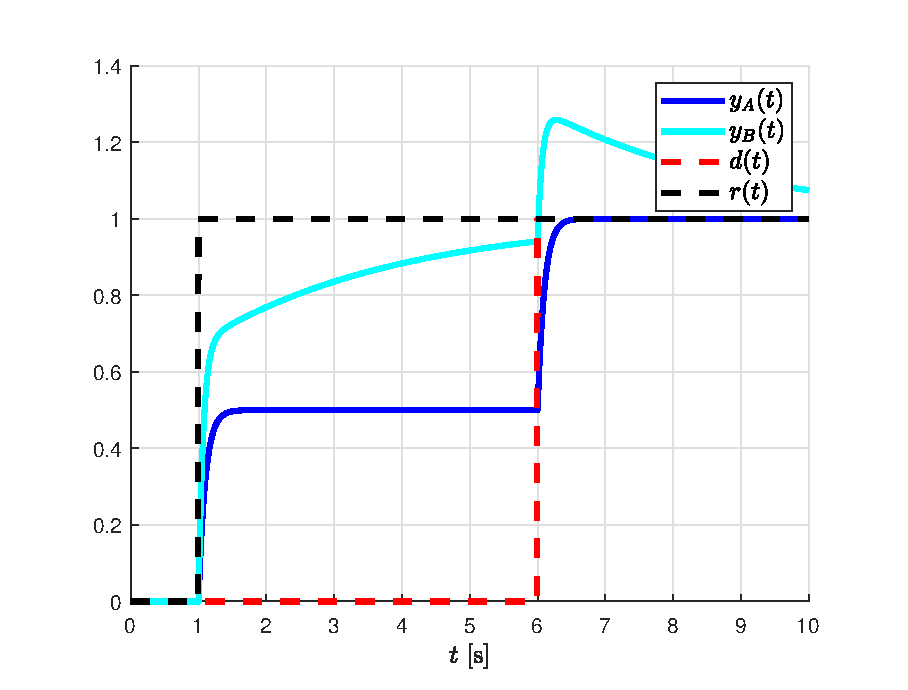
\includegraphics[width=\linewidth]{figs/fig7.eps}
        \caption*{(a): Respuesta del sistema}
    \end{minipage}
    \begin{minipage}{0.45\linewidth}
        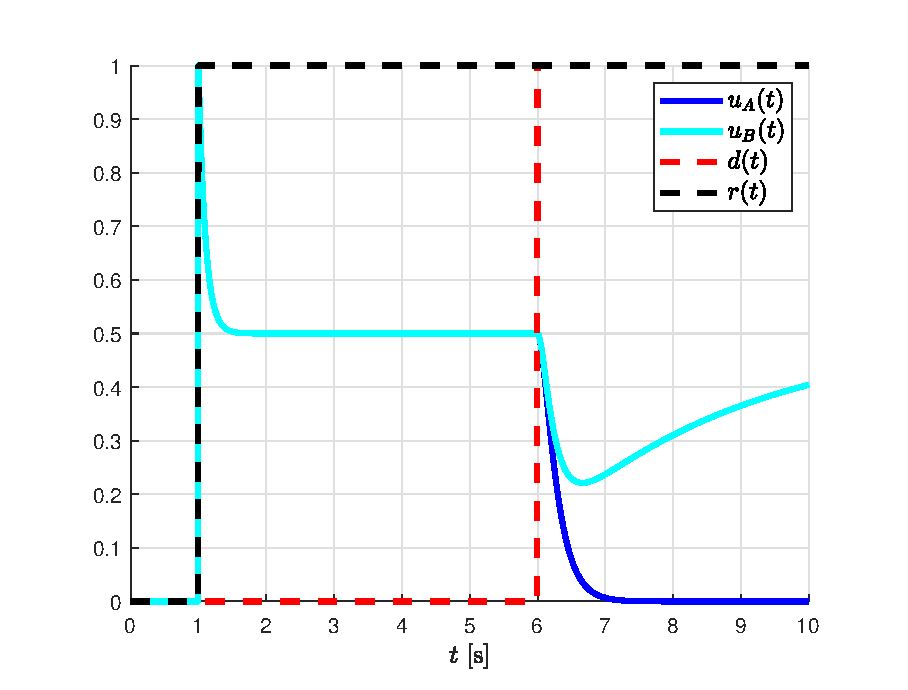
\includegraphics[width=\linewidth]{figs/fig6.eps}
        \caption*{(b): Respuesta del controlador}
    \end{minipage}
    \caption{Comparación de respuestas para ambos sistemas de control realimentados implementados con distintos controladores}
    \label{fig5}
\end{figure}

Como ya se mencionó anteriormente, el sistema de control realimentado implementado con el controlador de caracter integrante tiene mayor capacidad de rechazar los efectos de la perturbación sobre la salida del sistema. Esto se puede observar claramente en la figura anterior, ya que el controlador que es puramente proporcional no es capaz de que la respuesta del sistema llegue a la referencia por sí misma, y tampoco rechaza el efecto de la perturbación. Para explicar esto de mejor manera, se generaron los diagramas de polos y ceros para cada sistema realimentado. Se hizo por medio del siguiente código de MATLAB.

\vspace{1em}
\begin{mdframed}
\begin{minted}{matlab}
figure (7);
pzplot(MyrA, 'rO');

figure (8);
pzplot(MydA, 'rO');

pzplot(MydA, 'rO');

figure (9);
pzplot(MyrB, 'rO');

figure (10);
pzplot(MydB, 'rO');
\end{minted}
\end{mdframed}

\newpage

Se generaron los siguientes diagramas de polos y ceros.

\begin{figure}[!h]
    \centering
    \begin{minipage}{0.45\linewidth}
        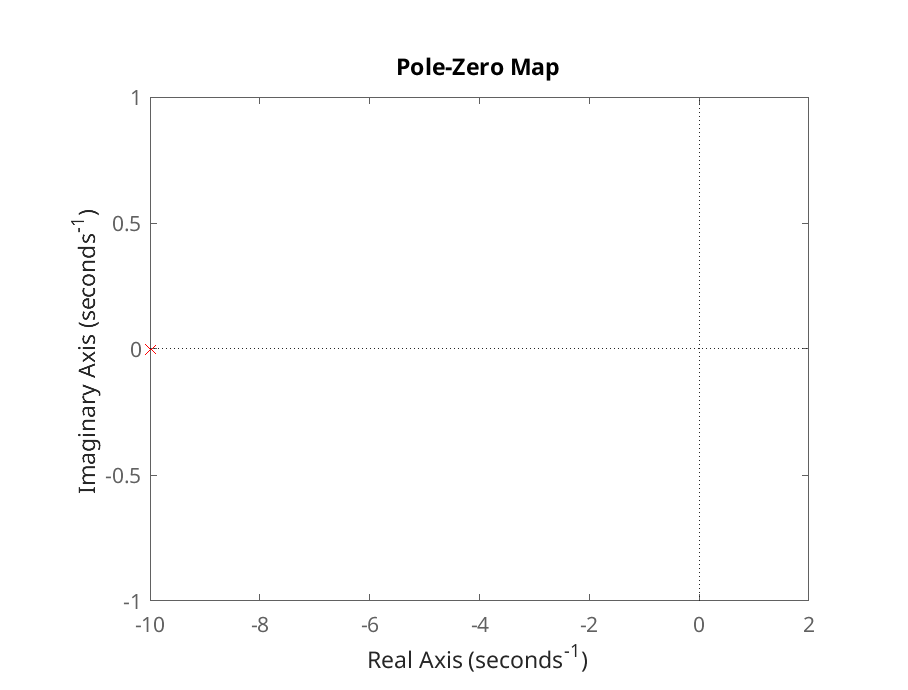
\includegraphics[width=\linewidth]{figs/fig8.eps}
        \caption*{(a): $M_{yr}(s)$}
    \end{minipage}
    \begin{minipage}{0.45\linewidth}
        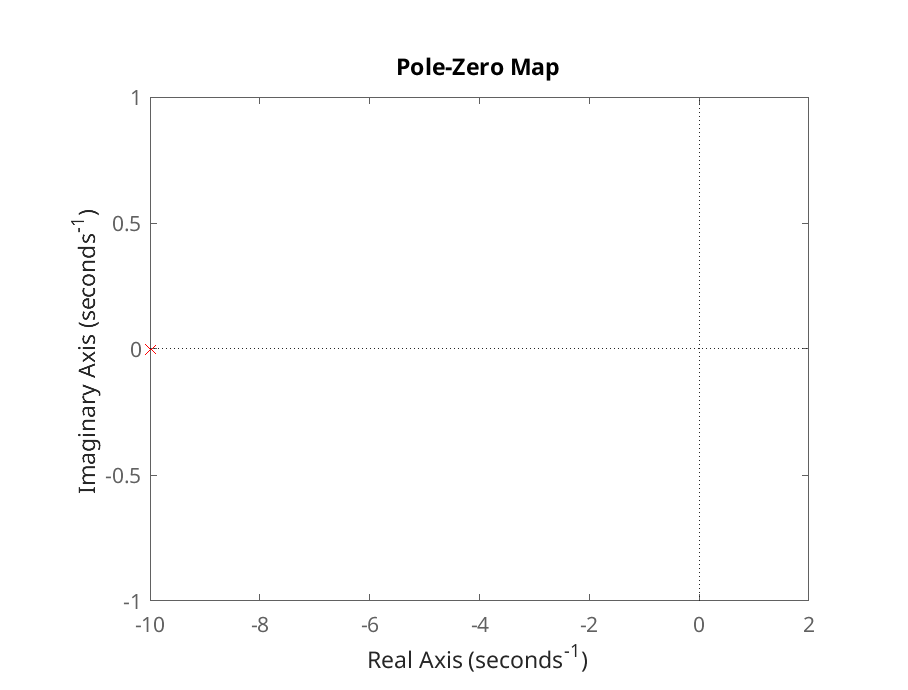
\includegraphics[width=\linewidth]{figs/fig9.eps}
        \caption*{(b): $M _{yd}(s)$}
    \end{minipage}
    \caption{Diagramas de polos y ceros del sistema de control realimentado con $C(s) = 1$}
    \label{fig6}
\end{figure}

\begin{figure}[!h]
    \centering
    \begin{minipage}{0.45\linewidth}
        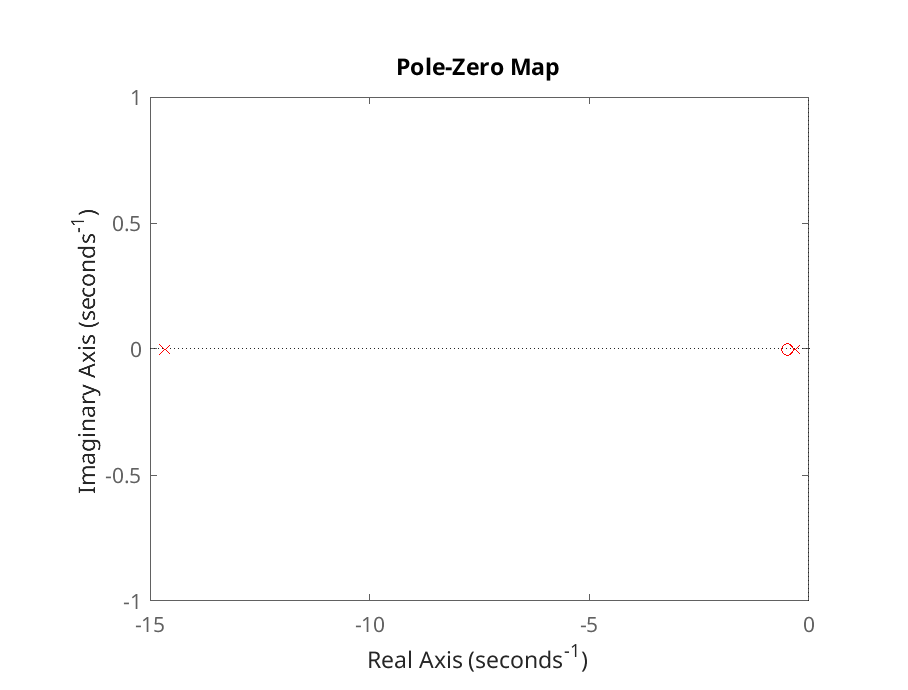
\includegraphics[width=\linewidth]{figs/fig10.eps}
        \caption*{(a): $M_{yr}(s)$}
    \end{minipage}
    \begin{minipage}{0.45\linewidth}
        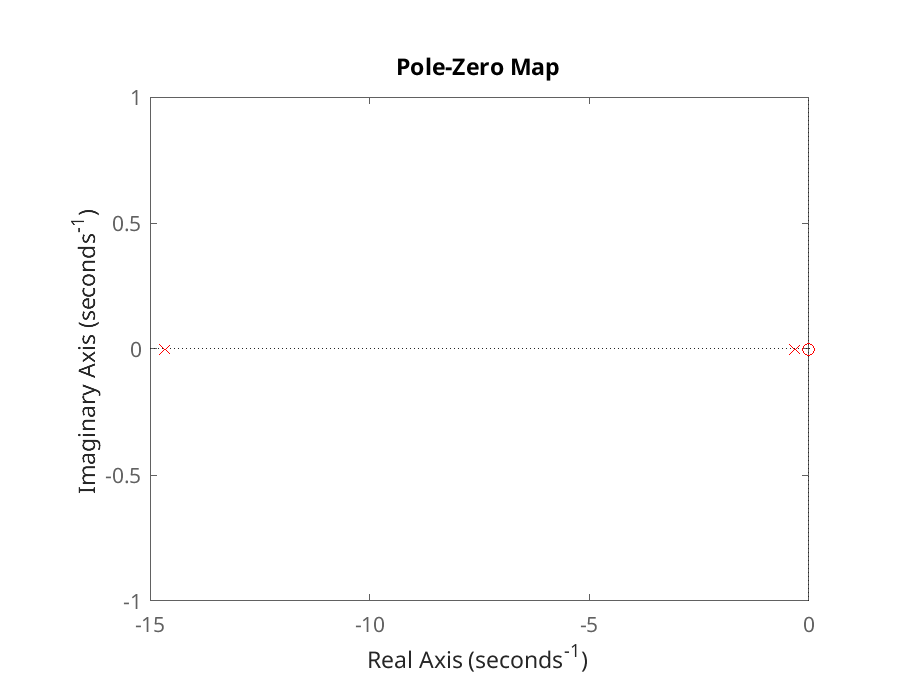
\includegraphics[width=\linewidth]{figs/fig11.eps}
        \caption*{(b): $M _{yd}(s)$}
    \end{minipage}
    \caption{Diagramas de polos y ceros del sistema de control realimentado con $C(s) = K_P(1 + 1/(sT_i))$}
    \label{fig7}
\end{figure}

La razón del porque el sistema se estabiliza a pesar de que el proceso sea integrador y no auto-regulado se debe a la acción integral del controlador. El polo que posee en el origen compensa el sistema no auto-regulado, eliminando el error estacionario. Esto asegura la estabilidad del sistema, lo cual no sucede con el controlador proporcional, ya que no posee un polo en el origen, implicando que el sistema no necesariamente será estable a largo plazo.

\vspace{1em}
\begin{mdframed}
        Así como el código fuente que genera este reporte y el código de MATLAB para generar las gráficas mostradas anteriormente se encuentran en el siguiente repositorio de Github:
    
    \begin{center}
        \href{https://github.com/Roger-505/tareas-ie0431}{\texttt{https://github.com/Roger-505/tareas-ie0431}}
    \end{center}
\end{mdframed}

